

\chapter{SoC与外设}

\section{概述}

我们致力于构建一套能提供\textbf{真正PC机体验}的SoC与外设系统。目前我们已驱动VGA、LCD、PS/2、GPIO、触摸、DDR、串口、以太网等一系列外设,初步达成了这一目标。其中,VGA、LCD、PS/2、GPIO的控制器和对应驱动为团队自行实现。

实机效果如图3.1所示。

%开始插入图片
\begin{figure}[htb] % htbp代表图片插入位置的设置
\centering %图片居中
%添加图片;[]中为可选参数,可以设置图片的宽高;{}中为图片的相对位置
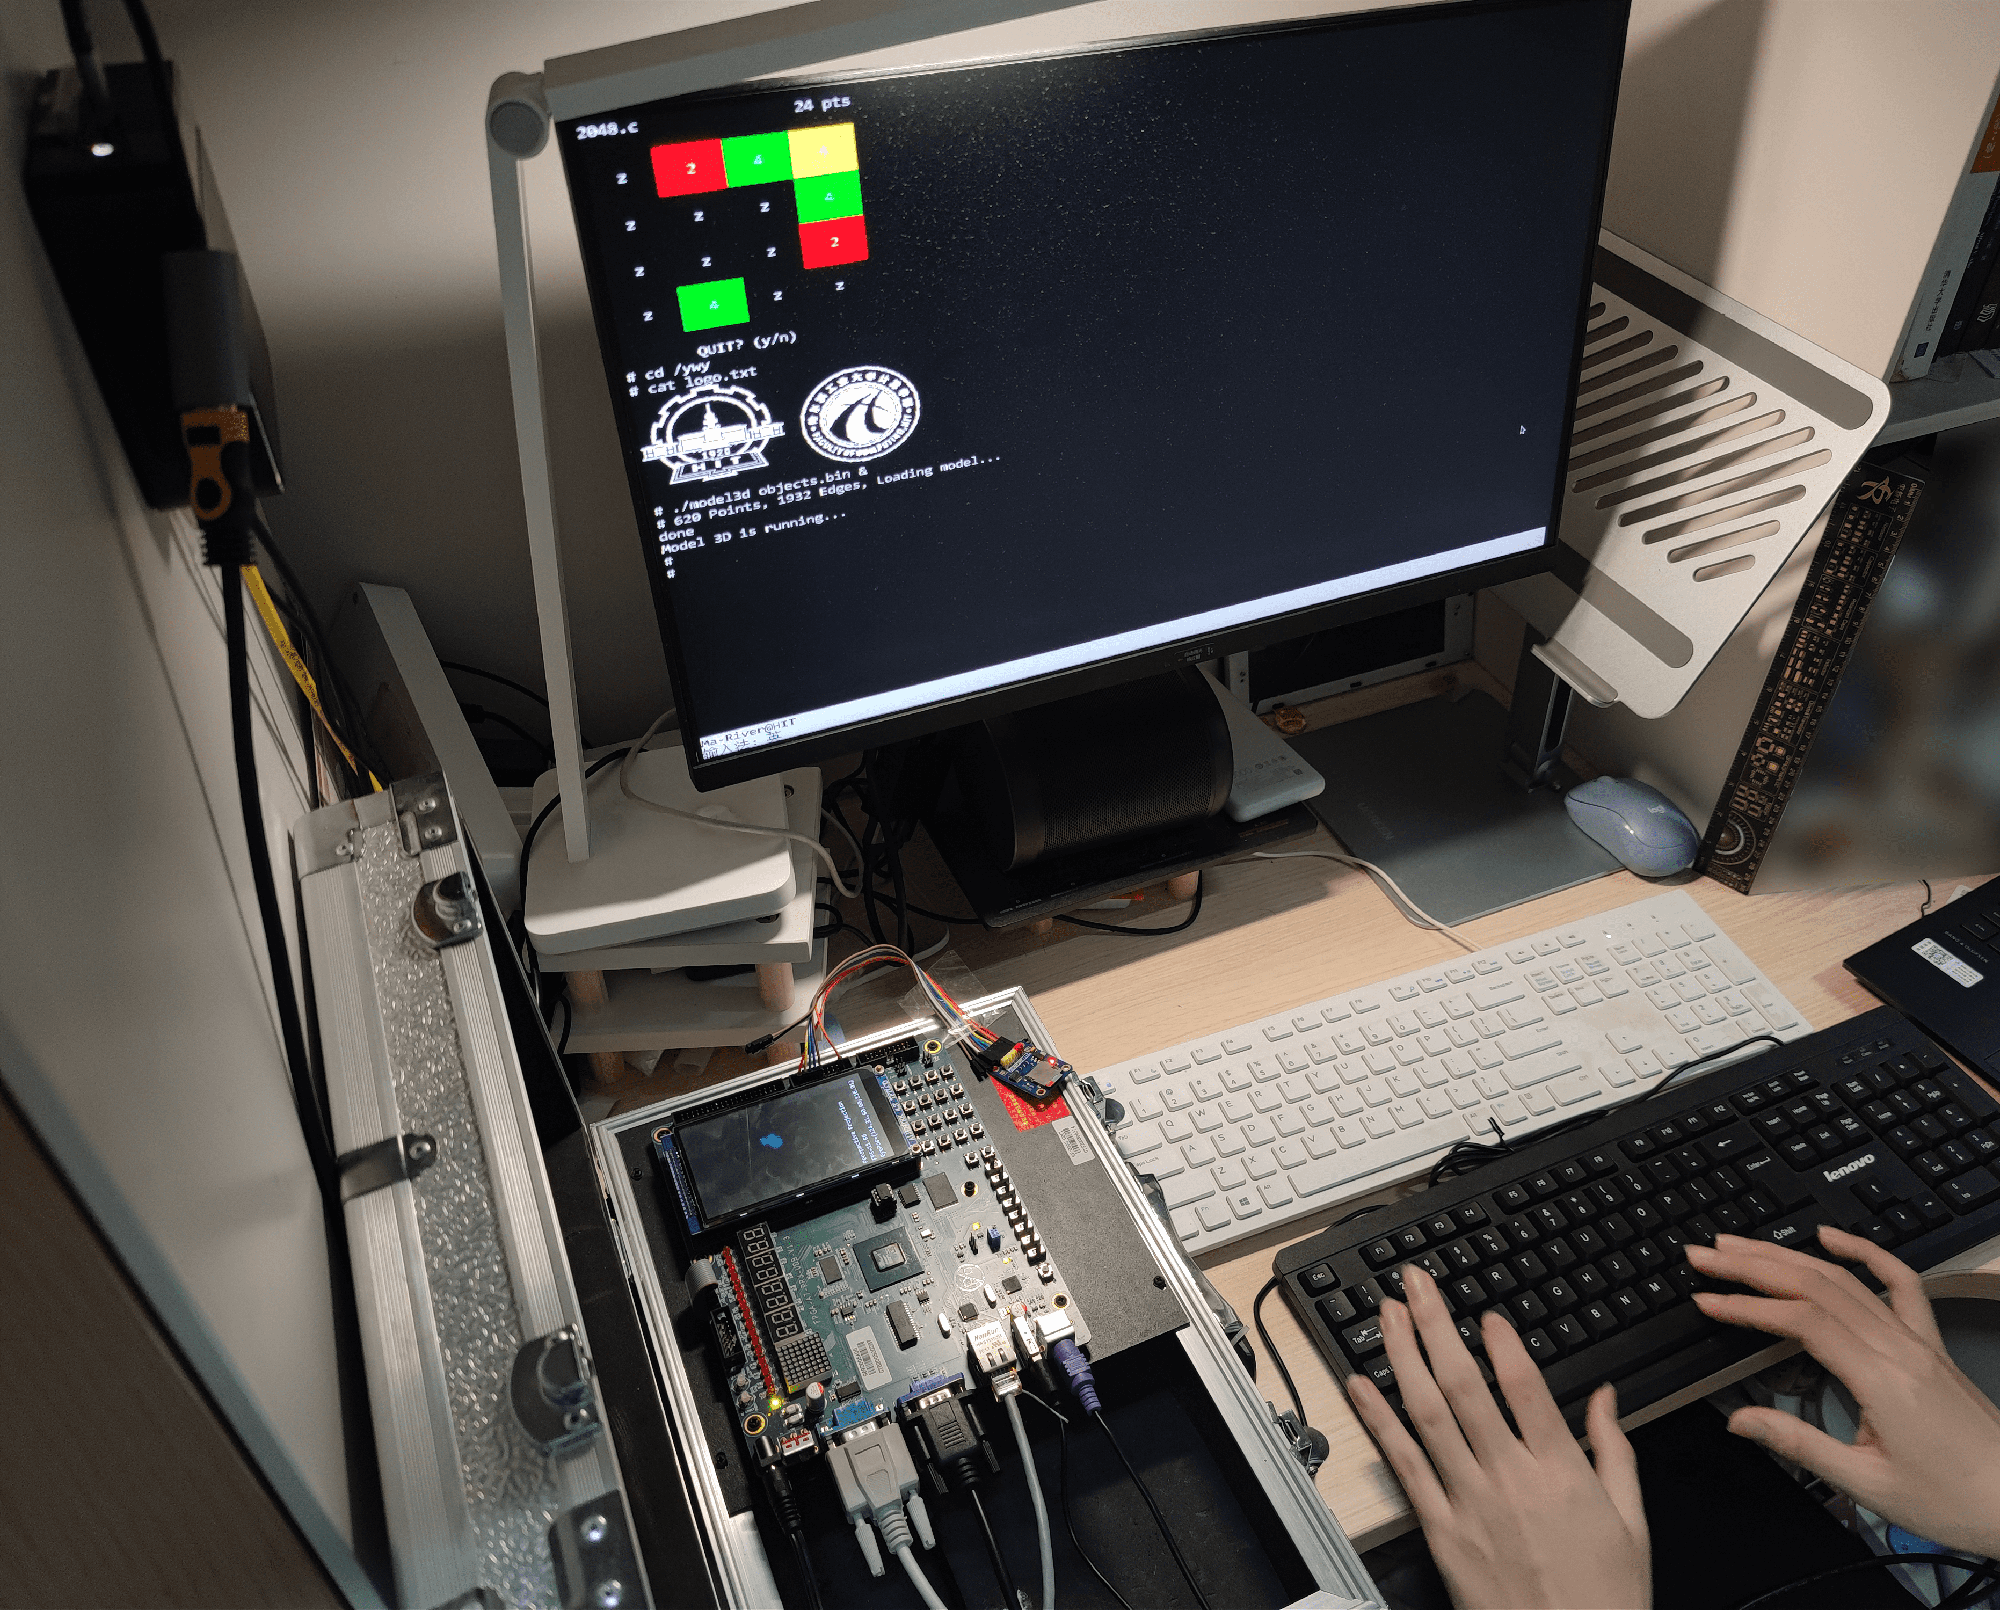
\includegraphics[width=12cm]{img/sys.png}
\caption{实机效果展示} % 图片标题
\label{pic1} % 图片标签
\end{figure}

\newpage

\section{整体架构}

SoC整体架构如下图所示:

\begin{figure}[!ht]
    \centering
    \begin{tikzpicture}[myrect/.style={rounded corners,draw=vivadodraw,fill=vivadofill}]
    
    
    \draw[myrect] (0,0) rectangle (235pt,30pt);
    \node[centered=0,font=\fontsize{9}{9}\selectfont,node font=\sffamily] (VGA) at (117.5pt, 15pt) {DDR};
    % 左半部分
    \draw[myrect] (0,45pt) rectangle (75pt,75pt);
    \draw[myrect] (0,90pt) rectangle (75pt,120pt);
    \draw[myrect] (0,135pt) rectangle (75pt,165pt);
    \draw[myrect] (0,180pt) rectangle (75pt,210pt);
    \draw[myrect] (0,225pt) rectangle (75pt,255pt);
    
    \node[centered=0,font=\fontsize{9}{9}\selectfont,node font=\sffamily] (VGA) at (37.5pt, 60pt) {VGA Controller};
    \node[above=45pt,centered=0,font=\fontsize{9}{9}\selectfont,node font=\sffamily] (USB) at (VGA) {USB Host Ctl};
    \node[above=45pt,centered=0,font=\fontsize{9}{9}\selectfont,node font=\sffamily] (IIC) at (USB) {AXI IIC};
    \node[above=45pt,centered=0,font=\fontsize{9}{9}\selectfont,node font=\sffamily] (Eth) at (IIC) {AXI EthernetLite};
    \node[above=45pt,centered=0,font=\fontsize{9}{9}\selectfont,node font=\sffamily] (INTC) at (Eth) {AXI INTC};
    
    % 中间
    \draw[myrect] (90pt,45pt) rectangle (145pt,255pt);
    \node[centered=0,font=\fontsize{9}{9}\selectfont,node font=\sffamily,align=center] at (117.5pt,150pt) {AXI \\
                   Interconnect};
    
    % 右半部分
    \draw[myrect] (160pt,45pt) rectangle (235pt,75pt);
    \draw[myrect] (160pt,90pt) rectangle (235pt,120pt);
    \draw[myrect] (160pt,135pt) rectangle (235pt,165pt);
    \draw[myrect] (160pt,180pt) rectangle (235pt,210pt);
    \draw[myrect] (160pt,225pt) rectangle (235pt,255pt);
    
    \node[centered=0,font=\fontsize{9}{9}\selectfont,node font=\sffamily] (LCD) at (197.5pt, 60pt) {LCD Controller};
    \node[above=45pt,centered=0,font=\fontsize{8.5}{8.5}\selectfont,node font=\sffamily] (BRAM) at (LCD) {Bootloader BRAM};
    \node[above=45pt,centered=0,font=\fontsize{9}{9}\selectfont,node font=\sffamily] (PS2) at (BRAM) {PS/2};
    \node[above=45pt,centered=0,font=\fontsize{9}{9}\selectfont,node font=\sffamily] (UART) at (PS2) {AXI UART};
    \node[above=45pt,centered=0,font=\fontsize{9}{9}\selectfont,node font=\sffamily] (GPIO) at (UART) {GPIO\&Clock};
    
    % 顶部
    \draw[myrect] (0pt,270pt) rectangle (235pt,300pt);
    \node[centered=0,font=\fontsize{9}{9}\selectfont,node font=\sffamily] (VGA) at (117.5pt, 285pt) {CPU};
    
    
    % AXI Master
    \draw[very thick,->] (117.5pt, 270pt) -- (117.5pt, 255pt); % CPU
    \draw[very thick,->] (37.5pt, 45pt) -- (37.5pt, 30pt); % VGA DMA
    \draw[very thick,->] (197.5pt, 45pt) -- (197.5pt, 30pt); % LCD DMA
    
    % AXI Slave
    \draw[thick,->] (90pt, 60pt) -- (75pt, 60pt);
    \draw[thick,->] (90pt, 105pt) -- (75pt, 105pt);
    \draw[thick,->] (90pt, 150pt) -- (75pt, 150pt);
    \draw[thick,->] (90pt, 195pt) -- (75pt, 195pt);
    \draw[thick,->] (90pt, 240pt) -- (75pt, 240pt);
    
    \draw[thick,->] (145pt, 60pt) -- (160pt, 60pt);
    \draw[thick,->] (145pt, 105pt) -- (160pt, 105pt);
    \draw[thick,->] (145pt, 150pt) -- (160pt, 150pt);
    \draw[thick,->] (145pt, 195pt) -- (160pt, 195pt);
    \draw[thick,->] (145pt, 240pt) -- (160pt, 240pt);
    
    \draw[thick,->] (117.5pt, 45pt) -- (117.5pt, 30pt);
    
    % Interrupts
    \draw[dashed,-latex] (0pt, 105pt) -- (-15pt, 105pt) -- (-15pt, 242pt) -- (0pt,242pt); % USB
    \draw[dashed,-latex] (0pt, 150pt) -- (-10pt, 150pt) -- (-10pt, 237pt) -- (0pt,237pt); % IIC
    \draw[dashed,-latex] (0pt, 195pt) -- (-5pt, 195pt) -- (-5pt, 231pt) -- (0pt,231pt); % Eth
    
    \draw[dashed,-latex] (235pt, 60pt) -- (255pt, 60pt) -- (255pt, 294pt) -- (235pt,294pt); % LCD
    \draw[dashed,-latex] (235pt, 150pt) -- (250pt, 150pt) -- (250pt, 288pt) -- (235pt,288pt); % PS/2
    \draw[dashed,-latex] (235pt, 195pt) -- (245pt, 195pt) -- (245pt, 282pt) -- (235pt,282pt); % UART
    \draw[dashed,-latex] (235pt, 240pt) -- (240pt, 240pt) -- (240pt, 276pt) -- (235pt,276pt); % GPIO
    
    \draw[dashed,-latex] (0pt, 248pt) -- (-15pt, 248pt) -- (-15pt, 285pt) -- (0pt,285pt); % INTC
    
    % 图注
    \draw[thick,->] (55pt, -10pt) -- (70pt, -10pt) node[right] {AXI总线};
    \draw[dashed,-latex] (140pt, -10pt) -- (155pt, -10pt) node[right] {中断};
    
    \end{tikzpicture}

    \caption{SoC整体架构} % 图片标题
    \label{pic_soc_all} % 图片标签
\end{figure}



\section{资源分配}

\subsection{外设地址}

\begin{table}[!ht]
\centering
\caption{设备物理地址分配}
\label{tab:pehi_addr}
\begin{tabular}{cc|cc}
\hline
设备名称           & 起始地址         & 设备名称                 & 起始地址                 \\ \hline
DDR3           & 0x0000\_0000 & VGA控制器               & 0x1FE0\_0000         \\
AXI IIC(触摸)    & 0x1FA0\_0000 & AXI UART16550        & 0x1FE4\_0000         \\
AXI INTC       & 0x1FB0\_0000 & AXI QUAD SPI     & 0x1FE8\_0000         \\
Bootloader ROM & 0x1FC0\_0000 & AXI Ethernetlite  &  0x1FF0\_0000                 \\
LCD控制器         & 0x1FD0\_0000 & \multicolumn{1}{l}{} & \multicolumn{1}{l}{} \\ \hline
\end{tabular}
\end{table}

\subsection{外设中断}

《MIPS指令系统规范》\footnote{参见龙芯杯2023发布包文档:《A03“系统能力培养大赛”MIPS指令系统规范v1.01》}中要求实现6个硬件中断,但计时器中断会复用 HW5 硬件中断,故可以直接使用的硬件中断只有5个,且仅支持电平触发中断;为了拓展中断数量、处理部分边沿触发的中断,我们使用了Xilinx AXI INTC IP核。

中断的连接关系如下图所示,其中AXI Ethernetlite为边沿触发中断,其他均为电平触发中断。

% Define color
\definecolor{vivadodraw}{rgb}{0.2549,0.3804,0.6235}
\definecolor{vivadofill}{rgb}{0.9294,0.9647,0.9960}


\begin{figure}[!ht]
    \centering
    
    \begin{tikzpicture}[myint/.style={anchor=east,inner sep=0,font=\fontsize{10}{10}\selectfont},node font=\sffamily]
    
    \draw[rounded corners,draw=vivadodraw,fill=vivadofill] (0, 0) rectangle (45pt, 140pt);
    
    \node[anchor=north] at (22.5pt, 0pt) {CPU INT};
    
    \node[myint] at (42pt, 120pt) {HW0};
    \node[myint] at (42pt, 100pt) {HW1};
    \node[myint] at (42pt, 80pt) {HW2};
    \node[myint] at (42pt, 60pt) {HW3};
    \node[myint] at (42pt, 40pt) {HW4};
    \node[myint] at (42pt, 20pt) {HW5};
    
    % \draw (45pt, 20pt) -- (55pt, 20pt) node[right] {保留};
    \draw (45pt, 100pt) -- (55pt, 100pt) node[right] {UART};
    \draw (45pt, 80pt) -- (55pt, 80pt) node[right] {GPIO\&Clock};
    \draw (45pt, 60pt) -- (55pt, 60pt) node[right] {LCD};
    \draw (45pt, 40pt) -- (55pt, 40pt) node[right] {PS/2};
    \draw (45pt, 20pt) -- (55pt, 20pt) node[right] {保留};
    
    
    \draw[->] (45pt, 120pt) -- (120pt, 120pt) -- (120pt, 100pt) -- (130pt, 100pt);
    
    \draw[rounded corners,draw=vivadodraw,fill=vivadofill] (130pt, 40pt) rectangle (175pt, 120pt);
    
    \node[anchor=north] at (152.5pt, 40pt) {AXI INTC};
    
    \node[myint] at (173pt, 100pt) {INTR0};
    \node[myint] at (173pt, 80pt) {INTR1};
    \node[myint] at (173pt, 60pt) {INTR2};
    
    \draw[blue,thick] (175pt, 100pt) -- (185pt, 100pt) node[right] {AXI Ethernetlite};
    \draw (175pt, 80pt) -- (185pt, 80pt) node[right] {AXI IIC};
    \draw (175pt, 60pt) -- (185pt, 60pt) node[right] {AXI QUAD SPI};
    
    \end{tikzpicture}

    \caption{中断的连接关系} % 图片标题
    \label{pic_intr} % 图片标签
\end{figure}



\section{外设说明}

\subsection{VGA}

实验板提供了标准VGA接口,我们为此自行设计并实现了具有文本和图像两种工作模式的VGA控制器,其分辨率和刷新率固定为1024×768@60Hz,位深度为4,能实现文本或图像的输出。

在文本模式下,VGA控制器按照8×16大小为一个格子,将屏幕划分为48行128列,每个格子可显示一个单色ASCII字符或半个汉字(两个格子显示一个汉字)。VGA控制器为ASCII字符内置了点阵字库,只需要通过AXI总线向对应地址写入颜色信息和字符的ASCII码即可显示对应的字符。为支持汉字等高级字符集,文本模式支持向格子中写入基于位的二值化图像信息(每个像素用一个位表示),只要在软件字库中添加自定义的点阵信息,即可显示任何语言的字符。此外,文本模式还具有可配置的闪烁光标。文本模式的全部图像信息直接使用片上BRAM存储,不需要消耗内存带宽,性能友好。

在图像模式下,无法直接在片上存储的图像数据只能通过DMA方式传输。VGA控制器会周期性地通过AXI总线从DDR中读取指定地址处的图像数据,显存地址和图像的显示区域由软件动态设置。基于图像模式和DMA机制,我们实现并移植了FrameBuffer驱动,能够实现虚拟终端、动画绘制、GUI应用等。

我们为U-Boot、ucore和Linux都移植了基于VGA控制器文本模式的Console驱动程序,使得用户可以直接使用VGA与系统进行交互。

\subsection{LCD及触摸}

实验板提供了分辨率为480*800的LCD屏幕,我们为其自行设计实现了LCD控制器实现文本与图像输出。LCD控制器也具有文本模式和图像模式。

LCD控制器的文本模式和VGA类似,故不再赘述。原则上系统Console也可使用LCD文本模式输出,但由于LCD屏幕太小,我们最终并未实现。

由于LCD本身具有显存,LCD的图像模式支持直接向屏幕某位置写入像素值,这会在单个像素上花费较多周期,CPU需要进行多次高代价uncached访存。为加速LCD图像绘制,我们也为LCD提供了DMA传输支持。软件可将像素数据准备在DDR中,设置LCD控制器的传输地址和范围即可启动单次DMA传输,LCD控制器会连续向显存中写入像素,传输完成后通过中断告知CPU。这使得我们基于LCD的动画应用可以以至少20~30FPS的帧率播放。基于其DMA机制,我们也实现并移植了和VGA类似的标准FrameBuffer驱动。

对于LCD的触摸功能,我们使用Xilinx AXI IIC IP核与LCD上的GT1151Q触摸芯片进行I2C通信,定时查询触摸状态,读取触摸坐标。

\subsection{PS/2键盘}

实验板提供了PS/2物理接口,我们为此自行设计并实现了简单的PS/2键盘控制器。它能够解析输入的PS/2物理信号,在按键按下或松开时发起键盘中断,读取来自键盘的扫描码。我们为键盘分配了单独的中断信号并将其连接到CPU的外部中断信号上,CPU可以通过AXI总线读取扫描码并响应中断。同时,我们使用了深度为4的FIFO对多个未读取的键盘扫描码进行缓冲。此外,对于不使用中断方式输入的系统(如U-Boot),可使用轮询方式读取扫描码。	

我们为PS/2键盘控制器编写了适配的驱动,结合VGA能达到实际PC机的体验。

\subsection{GPIO}
实验板上提供了LED、数码管、拨码开关、按键等GPIO设备,我们为此自行设计并实现了GPIO控制器以对它们进行读写以及可编程的中断控制。

\subsection{串口}
实验板提供了RS-232串行通信接口,我们使用官方提供的Xilinx UART16550进行驱动。该控制器的中断信号为电平触发,我们将其直接连接到CPU的外部中断信号上。

U-Boot和Linux源码中提供了相关驱动,可以直接使用。

\subsection{以太网}
实验板提供了以太网标准协议中的MDIO和MII接口。我们使用官方提供的Xilinx EthernetLite进行驱动。由于该IP仅提供上升沿触发的中断,我们使用中断控制器来转换中断类型。

U-Boot和Linux源码中提供了相关驱动,可以直接使用。

\subsection{SD卡}
我们通过实验板提供的拓展GPIO,连接了提供SPI接口的SD卡模块,故我们使用AXI QUAD SPI进行交互。

Linux源码中提供了相关驱动,可以直接使用。